\chapter{Experiments}
In this chapter, we provide more details on techniques used to gather the presented results. We also present more detailed and experimental results that lead us to the conclusions in previous chapter.

The original implementation provided with the research paper implements SSD in the \textit{Caffe} \footnote{\url{http://caffe.berkeleyvision.org/}} deep learning framework. We decided against performing our experiments in Caffe and decided to implement our version in newer \textit{PyTorch} \footnote{\url{https://pytorch.org/}} framework. 


\section{Xception}
In \cref{sec:fixxception} we introduced a hypothesis about Xception\textit{A}-SSD, and based on this hypothesis we presented the improved, Xception\textit{H} model. However, as suggested by the name, it was not our first modification, and we needed some trial-and-error testing to achieve this result.

We will describe every iteration of the Xception-SSD model we trained and the reasoning behind the individual modifications. For clarity, we will refer to the Xception\textit{X} models in this section only by their version letter. The performance of mentioned models on \textit{Surveillance dataset} is plotted on \cref{fig:xception_perf} and the feature map sizes inside the models are shown in \cref{tab:xmods}.


\begin{figure}
    \centering
    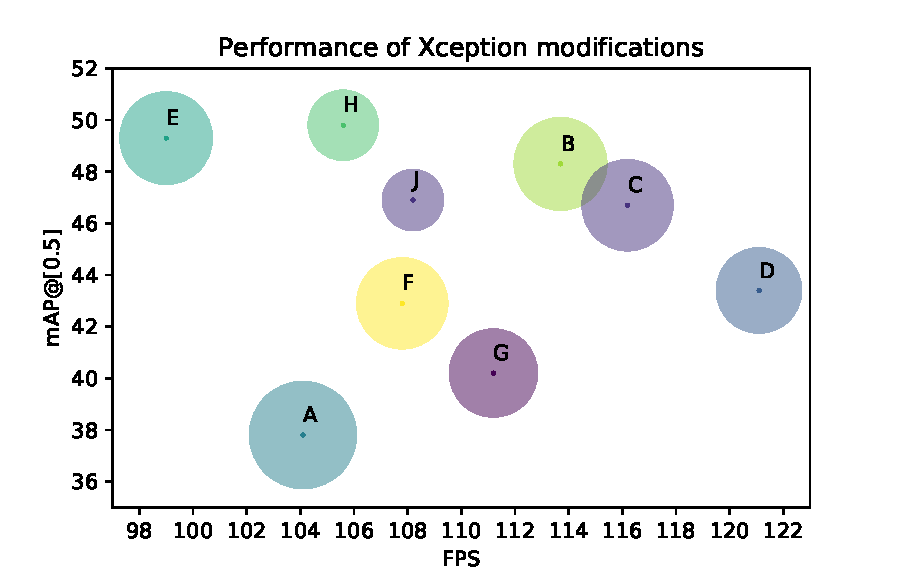
\includegraphics[width=0.95\textwidth]{img/fps_map_x}
    \caption[Performance of multiple Xception modification on Surveillance dataset]{Performance of multiple Xception modification on Surveillance dataset. Circle radii demonstrate relative difference of network parameter counts.} 
    \label{fig:xception_perf}
\end{figure}

\begin{table}[]
    \centering
    \begin{tabular}{c|c|c|c|c|c}
            &   A   &   B (C, D)   &   E (F, G)   &   H   &   J   \\
        \hline
        B1  &   [74\x128]   &   [74\x128]   &   [74\x128]   &   [74\x128]   &   [74\x128]   \\
        B2  &   \textbf{[37\x256]}   &  [37\x256]   &   [37\x256]   &   [37\x256]   &   [37\x256]   \\
        B3  &   [19\x728]   &   [19\x256]   &   [37\x256]   &   [37\x256]   &   [37\x256] \\
        \hline
        B4-6  &   [19\x728]   &   [19\x256]   &   [37\x256]   &   [37\x256]   &   [37\x256] \\
        B7  &   [19\x728]   &   \textbf{[19\x256]}   &   \textbf{[37\x256]}   &   \textbf{[37\x256]}   &   \textbf{[37\x256]} \\
        B8-10  &   [19\x728]   &   [19\x728]   &   [19\x728]   &   [19\x512]   &   [19\x512]\\
        B11 &   \textbf{[19\x728]}   &   \textbf{[19\x728]}   &   \textbf{[19\x728]}   &   \textbf{[19\x512]}   &   \textbf{[19\x512]}\\
        \hline
        B12 &   [10\x1024]  &   [10\x1024]  &   [10\x1024]  &   [10\x728]  &   [10\x512]\\
        S1  &   [10\x1536]  &   [10\x1536]  &   [10\x1536]  &   [10\x1024]  &   [10\x512]\\
        S2  &   \textbf{[10\x2048]}  &   \textbf{[10\x2048]}  &  \textbf{[10\x2048]}   &  \textbf{[10\x1024]} &  \textbf{[10\x512]}\\
    \end{tabular}
    \caption{Feature map sizes on the output of layers of the Xception networks. Bx stand for Xception blocks, S1 and S2 stand for separable convolution layers that follow the block structure (see \cref{fig:xception}). The first number represents spatial dimensions of a square feature, expecting [300\x300] input, and the second one represents the number of channels. The highlighted feature maps are used for the detections. The versions C, D and F, G share the feature maps sizes with their parent versions, if the given layers are present, but do not match the highlighted feature extraction.}
    \label{tab:xmods}
\end{table}

\subsubsection{Versions B, C, D}
We will take a look of this trio at once because version \textit{C} adds modifications to version \textit{B}, and version \textit{D} further modifies version \textit{C}. Notably, we trained these models in parallel and therefore had no results from concurrent models to inform on the design.

Starting with the assumption that the problem of the version \textit{A} is the location of the first feature extraction for detection, we moved the extraction from \textit{block 2} to \textit{block 7}. We also reduce the number of output filters on \textit{blocks 2 to 7} from 728 to 256. As a result the first detection is performed on a [19\x19\x256] feature map as opposed to original [37\x37\x256] map, but deeper in the network. 

Due to a reduction of feature map size, we considered this modification a half-measure in our plan to move the first feature extraction deeper into do network. However it proved to be a successful step in the right direction. The network has significantly gained in both speed and precision values. 

Both \textit{C} and \textit{D} were designed to observe the impact of removal of parts of the network and in no way modify parametrization of layers in the network. Version \textit{C} omits \textit{blocks 5, 6 and 7} and extracts the [19\x19] feature map after \textit{block 10} instead of \textit{block 11}. Version \textit{D}, was designed to test the need for 6 detection layers, mainly the layers for detecting large objects. It is based on \textit{C}, and removes the feature layers produced by \textit{extra layers}.

In version \textit{C}, we did not observe satisfying performance boost to justify received loss of precision. The version \textit{D}'s performance boost was more significant, however, it was coupled with major precision penalty.

\subsubsection{Versions E, F, G}
Similarly to the previous trio, these version are also based on each other, with \textit{E} being the main architectural change and versions \textit{F} and \textit{G} more of an independent experiments. 

Version \textit{E} is the one, where we finally implemented our original intention of moving first extracted feature map of [37\x37] size to a deeper layer. The only difference from \textit{B}, implementation-wise, is the movement of max-pooling with stride 2 from \textit{block 2} to \textit{block 8}. 

We can see a noticeable drop-off in performance compared to \textit{B}. Although the number of parameters in the network is the same, the change from [19\x19] to [37\x37] requires about 4 times more computation per convolutional layer. 


\subsubsection{Version H}

\subsubsection{Version J}


A - ap on person, car low


\section{Measurements}
To make our work comparable to other similar studies and future works, we present methods used for both precision and performance measurements.

\subsection{Precision}
Rather than implementing our own copy of the precision evaluation, all our precision measurements were taken using an external tool. Using the external tool, independent on our implementation, allows us to easily compare our results with other works with little to no modifications. We used the implementation by \citet{bib:metricsgit}, that mirrors the evaluation process of \textit{PASCAL VOC Challenge}. The default parameters were used, meaning that the interpolation of AP was calculated using all data points and the IoU threshold was set to 0.5. 

We present all the measurements taken on \textit{Surveillance dataset} while performing multiple experiments described in this thesis.


\begin{figure}
    \centering
    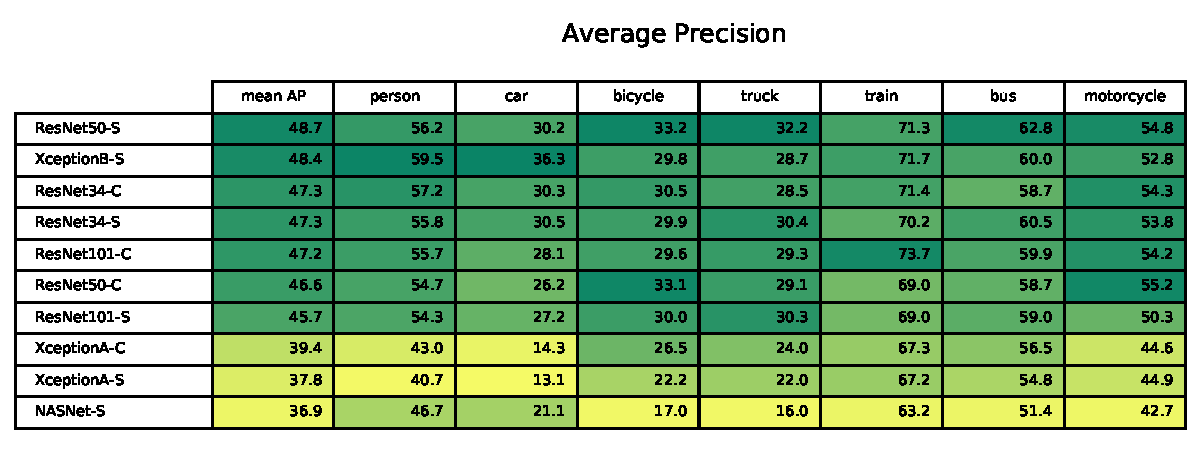
\includegraphics[width=\textwidth]{img/ap}
    \caption[Average precision of all tested networks on Surveillance classes]{Average precision of all tested networks on Surveillance classes. \textit{COCO} indicates that the network was trained on COCO dataset, otherwise only Surveillance data were used for training.} 
    \label{fig:ap}
\end{figure}

\subsection{Inference speed}
The absolute values of the inference speed measurement have no information value without the knowledge of the environment in which they have been taken. In this section, we provide the details of both software and hardware environments used for measurements.

The testing was done by timing the total time to process 10 000 images in batches of 16, and then simply calculating the \textit{fps} value. We do not consider scaling and cropping the images to be the part of the network and therefore we had no need to include this process in the measurement, the set of [300\x300] pixel images was pre-loaded into memory. On the other hand, the non-maximum suppression is critical part of the algorithm and is included. 

\paragraph{Hardware} All our testing was done on the following hardware:
\begin{itemize}
    \item AMD EPYC 7401P CPU @ 2GHz \x 24
    \item NVIDIA GeForce GTX 1080 Ti
    \item 128GB DDR4 RAM
\end{itemize}

\section{Training SSDTC}